\documentclass[tikz]{standalone}
% Preamble
	\usepackage{fullpage} % Package to use full page
	\usepackage{parskip} % Package to tweak paragraph skipping
	\usepackage{tikz} % Package for drawing
	\usepackage{amsmath}
	\usepackage{hyperref}
	\usepackage{amsmath,amssymb}
	\usepackage{color}
	\usepackage[version=4]{mhchem} 
	\usepackage{bm}
	\usepackage{verbatim}
	\usepackage{subfig}
	
	\usetikzlibrary{arrows,automata,positioning,backgrounds,calc,fadings}
	\usetikzlibrary{decorations.shapes}
	\usetikzlibrary{shapes,arrows,automata,positioning,fit,backgrounds,petri}
	\usetikzlibrary{fadings,decorations.pathmorphing}
	\usetikzlibrary{arrows,shapes}
	
	% Packages and code for framing
		\usepackage[framemethod=TikZ]{mdframed}
		%Theorem enviornment
			\newcounter{theo}[section]\setcounter{theo}{0}
			\renewcommand{\thetheo}{\arabic{section}.\arabic{theo}}
			\newenvironment{theo}[2][]{%
				\refstepcounter{theo}%
				\ifstrempty{#1}%
				{\mdfsetup{%
						frametitle={%
							\tikz[baseline=(current bounding box.east),outer sep=0pt]
							\node[anchor=east,rectangle,fill=blue!20]
							{\strut Theorem~\thetheo};}}
				}%
				{\mdfsetup{%
						frametitle={%
							\tikz[baseline=(current bounding box.east),outer sep=0pt]
							\node[anchor=east,rectangle,fill=blue!20]
							{\strut Theorem~\thetheo:~#1};}}%
				}%
				\mdfsetup{innertopmargin=10pt,linecolor=blue!20,%
					linewidth=2pt,topline=true,%
					frametitleaboveskip=\dimexpr-\ht\strutbox\relax
				}
				\begin{mdframed}[]\relax%
					\label{#2}}{\end{mdframed}}
		%Lemma enviornment 
			\newcounter{lem}[section]\setcounter{lem}{0}
			\renewcommand{\thelem}{\arabic{section}.\arabic{lem}}
			\newenvironment{lem}[2][]{%
				\refstepcounter{lem}%
				\ifstrempty{#1}%
				{\mdfsetup{%
						frametitle={%
							\tikz[baseline=(current bounding box.east),outer sep=0pt]
							\node[anchor=east,rectangle,fill=green!20]
							{\strut Lemma~\thelem};}}
				}%
				{\mdfsetup{%
						frametitle={%
							\tikz[baseline=(current bounding box.east),outer sep=0pt]
							\node[anchor=east,rectangle,fill=green!20]
							{\strut Lemma~\thetheo:~#1};}}%
				}%
				\mdfsetup{innertopmargin=10pt,linecolor=green!20,%
					linewidth=2pt,topline=true,%
					frametitleaboveskip=\dimexpr-\ht\strutbox\relax
				}
				\begin{mdframed}[]\relax%
					\label{#2}}{\end{mdframed}}	
		%Proof enviornment 
			\newcounter{prf}[section]\setcounter{prf}{0}
			\renewcommand{\theprf}{\arabic{section}.\arabic{prf}}
			\newenvironment{prf}[2][]{%
				\refstepcounter{prf}%
				\ifstrempty{#1}%
				{\mdfsetup{%
						frametitle={%
							\tikz[baseline=(current bounding box.east),outer sep=0pt]
							\node[anchor=east,rectangle,fill=red!20]
							{\strut Proof~\theprf};}}
				}%
				{\mdfsetup{%
						frametitle={%
							\tikz[baseline=(current bounding box.east),outer sep=0pt]
							\node[anchor=east,rectangle,fill=red!20]
							{\strut Proof~\thetheo:~#1};}}%
				}%
				\mdfsetup{innertopmargin=10pt,linecolor=red!20,%
					linewidth=2pt,topline=true,%
					frametitleaboveskip=\dimexpr-\ht\strutbox\relax
				}
				\begin{mdframed}[]\relax%
					\label{#2}}{\end{mdframed}}
%-------------
% Define different styles:
    %-------------
        \definecolor{deepskyblue}{cmyk}{1,0.25,0.0,0}
        \definecolor{picassoblue}{cmyk}{0.99,0.53,0.0,0.1}
    %-------------
        \tikzstyle{blue} = [circle,thick,inner color = picassoblue!100, outer color = deepskyblue!80, opacity = 0.9]
        \tikzstyle{vertex}=[rectangle,fill=white,minimum size=10pt,inner sep=0pt]
    %-------------					
\begin{document}
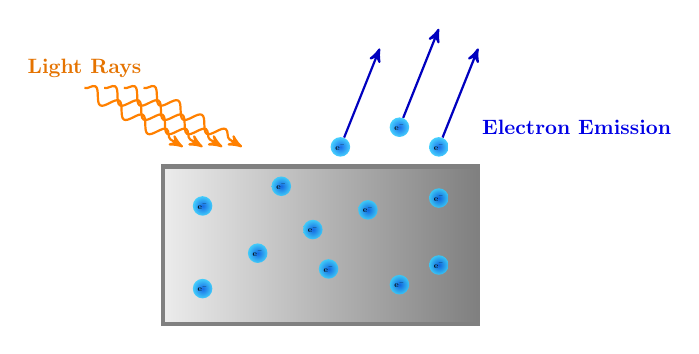
\begin{tikzpicture}[>=stealth',shorten >=0pt,auto,node distance=3cm,main node/.style={circle,thick, fill = white, scale=0.55, draw, font=\sffamily\large\bfseries}, photon/.style={decorate,decoration={snake,post length=1mm}}]
%-------------------------start grid code ---------------------
	%\def\figWd{8.5};
    %\def\figHt{8.5};
					
	%\draw[step=0.5,very thin, black!15] (-0.5,-0.5) grid (\figWd,\figHt);
	%\draw[thick,->] (0,0) -- (\figWd,0) node[anchor=north west] {$x$};
    %\draw[thick,->] (0,0) -- (0,\figHt) node[anchor=south east] {$y$};
					
	%\foreach \x in {0,...,\figWd} 
	%\draw (\x cm,1pt) -- (\x cm,-1pt) node[anchor=north] {$\x$};
	%\foreach \y in {0,...,\figHt}
    %\draw (1pt,\y cm) -- (-1pt,\y cm) node[anchor=east] {$\y$};
%--------------------------end grid code ----------------------
%--------------------start metal bar code ---------------------
	\filldraw[draw=gray, ultra thick, left color = white!85!gray, right color = gray] (2,2) rectangle (6,4);
					
	\coordinate (e1) at (2.5,3.5);
    \coordinate (e2) at (3.5,3.75);
	\coordinate (e3) at (4.6,3.45);
	\coordinate (e4) at (5.5,3.6);
	\coordinate (e5) at (3.2,2.9);
	\coordinate (e6) at (4.1,2.7);
	\coordinate (e7) at (3.9,3.2);
	\coordinate (e8) at (5,2.5);
	\coordinate (e9) at (2.5,2.45);
	\coordinate (e10) at (5.5,2.75);
					
	\node[blue,scale=0.3] (e1) at (e1) {\textcolor{black}{\textbf{\ce{e^-}}}};
	\node[blue,scale=0.3] (e2) at (e2) {\textcolor{black}{\textbf{\ce{e^-}}}};
	\node[blue,scale=0.3] (e3) at (e3) {\textcolor{black}{\textbf{\ce{e^-}}}};
	\node[blue,scale=0.3] (e4) at (e4) {\textcolor{black}{\textbf{\ce{e^-}}}};
	\node[blue,scale=0.3] (e5) at (e5) {\textcolor{black}{\textbf{\ce{e^-}}}};
	\node[blue,scale=0.3] (e6) at (e6) {\textcolor{black}{\textbf{\ce{e^-}}}};
	\node[blue,scale=0.3] (e7) at (e7) {\textcolor{black}{\textbf{\ce{e^-}}}};
	\node[blue,scale=0.3] (e8) at (e8) {\textcolor{black}{\textbf{\ce{e^-}}}};
	\node[blue,scale=0.3] (e9) at (e9) {\textcolor{black}{\textbf{\ce{e^-}}}};
	\node[blue,scale=0.3] (e10) at (e10) {\textcolor{black}{\textbf{\ce{e^-}}}};
%---------------------end metal bar code-----------------------
%--------------------start light rays code ---------------------
	\coordinate (label1) at (1,5.25);
	\node[vertex,scale=0.75] (label1) at (label1) {\textcolor{orange!90!black}{\textbf{Light Rays}}};
										
	\foreach \x in {0,0.25,...,0.75}
		{\coordinate (x1) at (1 + \x, 5);
			\coordinate (x2) at (2.25 + \x, 4.25);
			\draw[->,photon,color=orange,thick] (x1) -- node[above left] {} (x2);
		};				
%---------------------end light rays code -----------------------
%--------------------start emitted electrons code ---------------------	
	\coordinate(E1_start) at (4.25, 4.25);
	\coordinate(E1_end) at (4.75, 5.5);					
	\node[blue,scale=0.3] (E1_start) at (E1_start) {\textcolor{black}{\textbf{\ce{e^-}}}};
	\path[->][black!25!blue,thick] (E1_start) edge [bend left=0] node{} (E1_end);
					
	\coordinate(E2_start) at (5, 4.5);
	\coordinate(E2_end) at (5.5, 5.75);					
	\node[blue,scale=0.3] (E2_start) at (E2_start) {\textcolor{black}{\textbf{\ce{e^-}}}};
	\path[->][black!25!blue,thick] (E2_start) edge [bend left=0] node{} (E2_end);
					
	\coordinate(E3_start) at (5.5, 4.25);
	\coordinate(E3_end) at (6, 5.5);					
	\node[blue,scale=0.3] (E3_start) at (E3_start) {\textcolor{black}{\textbf{\ce{e^-}}}};
	\path[->][black!25!blue,thick] (E3_start) edge [bend left=0] node{} (E3_end);
					
	\coordinate (label2) at (7.25,4.5);
	\node[vertex,scale=0.75] (label2) at (label2) {\textcolor{blue!90!black}{\textbf{Electron Emission}}};
%---------------------end emitted electrons code ----------------------
\end{tikzpicture}
\end{document}
				